\section{Implementation}
\label{sec:impl}
Our approach to the DNS rebinding attack is derived from a standard time-varying attack, which can potentially take several minutes based on browser implementation of DNS Pinning. We discovered a previously undocumented variation which takes on the scale of tens of seconds. Instead of waiting for the pinned entries to expire, we flood the DNS cache with enough invalid entries to remove valid entries from the list. We plan to build on this idea and provide the attacker with a seamless browsing experience on the victim's internal server. We will retrieve the data from the victim's server (similar to existing scraping methods). Then we will allow the attacker to click links, take actions, and submit forms by sending the data to the victim's browser (which is acting as a proxy) and instruct it to send the appropriate request to the server.

%use this:
Reference the figure like this: Figure \ref{fig:firedrill1}.

\begin{figure}[h]
\centering
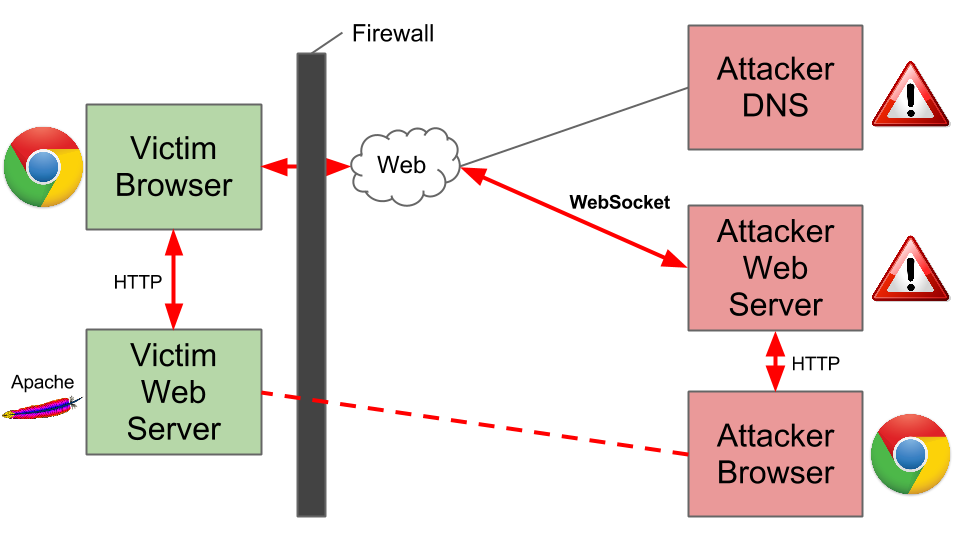
\includegraphics[width=0.8\columnwidth]{firedrill1.png}
\caption{\textbf{FireDrill Attack Overview.} When a victim accesses the attacker's web server, a malicious Javascript payload is delivered to be run on the victim's Browser. It then issues a large amount of DNS request to flood victim's DNS table and rebind the original domain name to the IP address of Victim's Web Server. The victims' browser then becomes a proxy between the internal websites and the attacker's browser. The attacker can navigate it like regular websites}
\label{fig:firedrill1}
\end{figure}

\subsection{Malicious DNS server}
Our system consists of a custom DNS server authoritative for the domain name takenoteswith.us. The DNS server keeps track of DNS requests and their source IP address. When the DNS server sees a request for the first time, it returns a IP address \textbf{54.224.61.225}, which is the address of our apache web server. If the DNS server has seen the DNS requests from the same ip address twice or more, it knows that this DNS requests is initiated by the rebinding script. At this time, the the malicious DNS server will return an IP address of \textbf{127.0.0.1}(Or whatever the attacker wants), which is the IP that the attacker wants it to bind to.

\subsection{Rebinding based on DNS table flooding}
To remove a pinned entry from the DNS entry table, we use DNS flooding technology. In current implementation of Chrome, all the domain names that are in the same level have the same priority. For this reason, we set our malicious URL(The URL that we ask the user to click in) to \textbf{n1.takenoteswith.us}.
We then flood the DNS table using DNS records from \textbf{n2.takenoteswith.us} to \textbf{n120.takenoteswith.us} (In this case, we assume the browser's DNS table size is 100)The number of bogus DNS requests are slightly more than 100 here because we want to speed up the process by eliminating the tail effects.

The careful readers may find that the request should not have completed since they disobey the same origin policy. However, the Chrome browser will still put the bogus entry in the DNS cache table and treat them with the same priority. 

\subsection{Malicious Javascript proxy}
The malicious Javascript proxy will be run on the victim's browser. It builts a Websocket connection to the attacker's webserver and receives proxy commands from it. The commands from the webserver have three fields, the \textbf{method} field is used to specify whether a post or get request should be forwarded. The \textbf{url} field specify the target of the request. The \textbf{args} field contains the arguments of the request.

The response from the Javascript proxy to the server is a little bit tricky. Other than plain HTML, sometimes the attacker wants to achieve binary data like photos and audios. In this case, the proxy has to put the HTTP headers('content-type', specifically) into the response so that the attacker's browser knows how to parse it. If the response is compressed, the Javascript is asked to decompress it. In this case, the HTTP header field 'content-length' should be changed accordingly. Lastly, if the response contains binary data, the Javascript is asked to encode it using base64 so that it can be transmitted in a JSON object. 

\subsection{Attacker's interface}
When a victim is connected, a new session is created and the attacker will get notified via both a webpage or Email. The attacker can access the interactive session using his/her browser like regular websites. 

When the attacker request a web object, it sends a request to his/her webserver that is connected to the victim's browser. The webserver will spawn a thread to handle the request. What the thread does is it will forward the request to the Javascript proxy, sleep and wait for the request then wake up again when the response from the proxy is available. The thread then decode the response, rebuild the HTTP header, then forward it back to the browser it is connected to.
